\def\radiusneuron{0.2cm}
\def\radiussynapse{0.02cm}
\def\lendens{0.5cm}
\def\lenax{2cm}
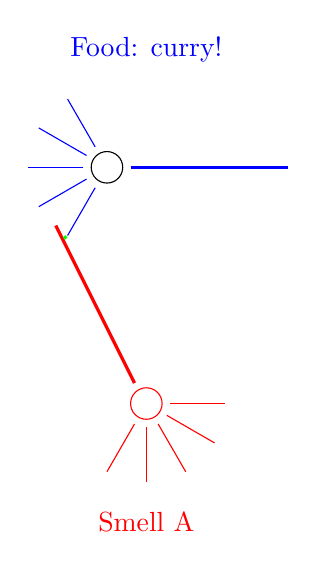
\begin{tikzpicture}[scale=1, transform shape]
  % Neuron 1
  \def\circlex{1.5}
  \def\circley{0}
  \draw [red] (\circlex, \circley) circle (\radiusneuron);
  \foreach \angle in {240, 270,...,360} \draw [red] ([shift=(\angle:\radiusneuron + 0.1cm )] \circlex, \circley) -- ++ (\angle:\radiusneuron+\lendens);
  \draw [red, very thick] ([shift=(120:\radiusneuron + 0.1cm )] \circlex, \circley) -- ++ (-1cm, \lenax);
  \node [red] at (\circlex, \circley - 1.5) {Smell A};
  \node [blue] at (\circlex, 3 + 1.5) {Food: curry!};

  % Neuron 2
  \def\circlex{1}
  \def\circley{3}
  \draw (\circlex, \circley) circle (\radiusneuron);
  \foreach \angle in {120, 150,...,240} \draw [blue] ([shift=(\angle:\radiusneuron + 0.1cm )] \circlex, \circley) -- ++ (\angle:\radiusneuron+\lendens);
  \draw [blue, very thick] ([shift=(0:\radiusneuron + 0.1cm )] \circlex, \circley) -- ++ (\lenax, 0);

  % Synapse
  \def\circlex{0.47}
  \def\circley{2.11}
  \draw [green, fill=green] (\circlex, \circley) circle (\radiussynapse);
\end{tikzpicture}

